%!TEX root = ../sztuthesis_main.tex

\section{引言}

\subsection{研究背景与意义}
随着数字音乐平台、音乐推荐系统和多媒体内容理解技术的快速发展，如何从音乐音频中自动提取高层语义信息并进一步完成情感分析，已经成为音乐信息检索领域的重要研究方向。与语音信号不同，音乐音频通常同时包含旋律、节奏、和声、音色、配器和风格等多层次信息，其情感表达具有较强的抽象性与主观性。因此，音乐情感分析不仅涉及低层声学信号处理，还涉及音乐语义理解、情绪建模和结果解释等问题。

传统音乐情感分析方法大多以梅尔频率倒谱系数、频谱特征、节奏特征等声学特征为输入，再结合支持向量机、线性回归、随机森林或神经网络等模型完成情感预测。这类方法在结构上较为清晰，在特定数据集上的数值预测也具备一定稳定性，但其主要局限在于：模型往往直接从特征映射到标签，难以显式刻画音乐中的旋律走向、节奏风格和整体听感等高层语义信息；当模型输出某种情感结果时，也较难回答“为什么这段音乐会被判定为该情感”这一问题。

近年来，大语言模型和多模态大模型在文本理解、结构化推理和音频语义建模方面展现出了较强能力。这为音乐情感分析提供了新的思路，即不再直接从音频信号端完成情感预测，而是先将音乐音频转换为自然语言描述，再利用大语言模型完成情感推理。通过引入“音频描述”这一中间语义层，可以将音乐中隐含的旋律、节奏、乐器和整体氛围信息显式表达出来，从而提升系统的可解释性和分析能力。

基于上述背景，本文围绕“基于大语言模型的音乐音频信号描述与情感标签生成”这一课题开展研究，尝试构建一条从音乐音频输入到文本描述生成，再到情感维度与情感标签输出的完整处理链路。从本科毕业设计的角度看，这一课题既具有一定研究意义，也具备较强工程实现价值：一方面，它能够体现音频处理、多模态模型调用、大语言模型推理和实验分析等多方面技术；另一方面，它也能够形成较完整的系统流程，为毕业论文写作和后续优化提供扎实基础。

\subsection{国内外研究现状}
从现有研究路线来看，音乐情感分析方法大致可以分为三类。第一类是基于传统声学特征和机器学习模型的方法。该类方法通常通过频谱、节奏、能量、音高等特征构建数值表示，再完成回归或分类任务，具有实现流程清晰、训练成本较低等特点。第二类是基于深度学习的端到端方法。这类方法通常将频谱图、波形或时频表示输入卷积神经网络、循环神经网络或 Transformer 结构中，直接学习从音频到情感标签之间的映射关系。第三类则是近年来逐渐出现的多模态与大模型方法，即利用具备音频理解能力的模型获得更高层语义表示，再通过语言模型完成解释、问答、摘要或推理任务。

相较于前两类方法，基于大模型的路线目前仍处于探索阶段。其优势在于能够更好地利用自然语言这一中间表示来组织音乐语义，从而为复杂的情感判断提供解释线索；但与此同时，这类方法也面临输出稳定性不足、提示词敏感、实验成本较高以及评估方式尚不统一等问题。因此，如何将大模型能力与音乐情感分析任务有效结合，仍然是一个值得进一步研究的问题。

从当前公开研究和工程实践来看，直接面向音乐内容生成描述文本并进一步完成情感推理的工作还不算充分，尤其是在本科毕业设计层面，围绕公开数据集搭建完整实验链路并对中间结果进行分析的研究更具实践价值。基于这一判断，本文没有选择完全端到端的黑盒预测路线，而是采用“音频描述中间层 + 大语言模型情感推理”的两阶段方案，希望在保证系统可运行的同时，提高整个过程的可解释性。

\subsection{研究目标与任务书要求}

围绕 DEAM 音乐情感数据集，构建一套结构完整、流程规范的音乐情感分析实验体系，实现从音频信号输入到情感结果输出的端到端处理流程。该体系涵盖音频数据预处理、音乐内容描述生成、情感维度推理以及对比实验分析等关键环节，以支撑后续方法评估与结果分析。

结合课题任务书要求，具体研究任务可归纳如下。

（1）音频数据整理与预处理。对原始音乐音频及其对应的情感标注数据进行系统整理，完成音频格式统一、重采样、静音裁剪、音量归一化等预处理操作，并构建结构化元数据。同时，依据实验需求完成训练集、验证集与测试集的划分，以保证数据使用的规范性与实验结果的可复现性。
（2）音乐音频描述生成方法设计。构建音频到文本的映射流程，基于预训练音频理解模型对音乐片段进行语义解析，生成结构化的中文描述文本。所生成描述需覆盖旋律、节奏、乐器、曲风及整体听感等关键维度，以增强中间表示的可解释性。
（3）情感推理模型构建。以生成的文本描述作为输入，构建基于大语言模型的情感推理模块，输出与 DEAM 标注体系对齐的 Valence 与 Arousal 连续情感维度值，并通过统一映射函数将连续空间划分为离散情感类别，实现多粒度情感表达。
（4）对比实验与基线方法构建。引入基于传统声学特征的机器学习方法作为对照基线，完成连续情感预测与离散情感分类任务，并在统一评价指标与标签映射规则下，与大语言模型方法进行对比分析，以验证不同方法在当前任务中的表现差异。

\begin{figure}[htbp]
    \centering
    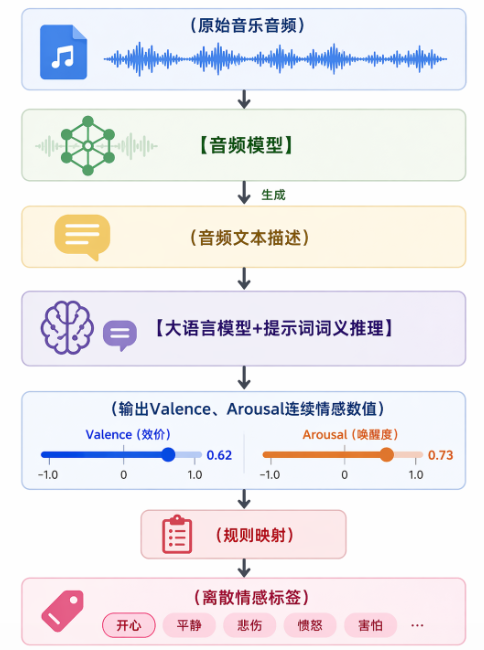
\includegraphics[width=0.65\linewidth]{image.png}
    \caption{音乐情感分析技术路线}
    \label{fig:tech_pipeline}
\end{figure}

图 \ref{fig:tech_pipeline} 展示了整体技术路线。该流程以原始音乐音频为输入，经由音频理解模型生成文本描述，再通过大语言模型进行语义推理，输出 Valence 与 Arousal 连续情感数值，最终通过规则映射得到离散情感标签。该设计在保证情感预测能力的同时，引入中间文本表示以提升系统的可解释性。

从当前阶段性实验结果来看，已完成主流程在测试集上的贯通实现，即能够在与基线方法一致的数据划分与评价口径下，由音频输入生成对应的中文描述，并进一步完成情感维度的批量推理。相关实验结果通过统一评价脚本进行统计，并输出汇总指标、逐样本结果及可视化分析结果。

整体而言，当前研究已实现“流程可运行、结果可对齐、实验可复现”的阶段性目标。后续工作将重点围绕提示词设计优化、情感建模细化以及评价方法完善等方面展开，以进一步提升模型性能与分析深度。

\subsection{研究内容与技术路线}
本文的整体技术路线可以概括为：首先读取 DEAM 数据集中的音频与静态情感标注，并完成标准化预处理；随后根据 Valence 和 Arousal 值对样本进行分层划分，构建训练集、验证集与测试集；接着利用预训练音频理解模型对测试音频生成中文文本描述；在得到描述文本后，使用大语言模型对描述进行情感推理，输出 Valence、Arousal 和离散情感标签；与此同时，构建基于传统声学特征的机器学习基线，并与大模型方法进行对比；最后对实验结果进行统计、可视化和误差分析。

从系统结构上看，本文主要包含数据预处理模块、音频描述生成模块、描述质量评估模块、情感推理模块、传统基线模块和结果分析模块六个部分。其中，音频描述生成与情感推理共同构成本文的核心两阶段框架，而传统基线模块则主要作为对照实验存在。通过这样的设计，本文既能够展示一条以大模型为核心的新路径，也能在实验中与经典方法形成横向比较。

\subsection{论文结构安排}
全文共分为六章，各章内容安排如下。

第一章为引言，主要介绍研究背景、研究现状、研究目标、技术路线及论文结构。

第二章为数据集构建与预处理，重点介绍 DEAM 数据集、情感标注体系、音频预处理流程以及训练集、验证集和测试集的划分方法。

第三章为音频到文本描述生成方法，主要介绍预训练音频理解模型的选型思路、云端调用实现、提示词设计以及描述质量评估方法。

第四章为基于大语言模型的情感推理方法，重点介绍情感推理任务建模、模型接口实现、提示词模板设计、批量推理流程以及情感标签组织策略。

第五章为对比实验与结果分析，主要对大模型链路和传统声学特征机器学习基线进行实验比较，并进一步分析当前系统存在的误差来源与局限性。

第六章为总结与展望，对全文工作进行总结，并提出后续可进一步改进的方向。

\newpage

\section{数据集构建与预处理}

\subsection{音乐数据集选型与标注体系}
本研究围绕“基于大语言模型的音乐音频信号描述与情感标签生成”这一任务展开。为了保证实验数据具有较好的代表性与可用性，课题选用了 DEAM（Database for Emotional Analysis of Music）数据集作为主要研究对象。该数据集是音乐情感计算领域中较为常用的公开数据集之一，包含大量音乐片段及对应的情感标注信息，能够为音乐情感分析相关研究提供较为统一的数据基础。

选择 DEAM 数据集的主要原因有以下几点。首先，该数据集面向音乐情感分析任务构建，数据内容与本文研究方向高度一致。其次，数据集中提供了情感维度标注，适合用于建立从音乐内容到情感结果的映射关系。再次，DEAM 数据集同时包含音频数据与情感标注文件，便于构建从原始音频输入到情感推理输出的完整实验链路。同时，使用公开数据集还能够降低数据采集和人工标注的工作成本，使研究重心集中在方法实现与实验分析上。

在情感表示方式上，本文采用 Valence-Arousal 二维情感模型对音乐情感进行描述。其中，Valence 表示情绪的愉悦程度，通常反映音乐给人带来的正向或负向感受；Arousal 表示情绪的唤醒程度，反映音乐在情绪强度上的活跃或平缓特征。与仅使用“快乐”“悲伤”等离散标签相比，Valence-Arousal 模型能够更细致地描述音乐情感状态，因而在音乐情感计算任务中具有较高的适用性。

从项目实现角度看，当前系统主流程主要使用 DEAM 数据集中的静态情感标注信息，即每首歌曲对应的平均 Valence 与平均 Arousal 数值，作为后续样本构建与实验评估的基础。系统中虽然也实现了对动态逐秒标注文件的读取与验证，但从当前主流程来看，动态标注尚未纳入描述生成与情感推理实验之中。因此，本文的主要实验对象为基于歌曲级静态标注的音乐情感分析任务。

结合当前系统实现可以看出，项目将每个可用音频样本与其对应的情感标注一一对齐，并在后续处理中保留样本编号、音频路径以及对应的 Valence 和 Arousal 均值等关键信息。这种组织方式为后续的音频描述生成、情感推理以及与传统基线方法的对比实验提供了统一的数据接口，也使得整个实验链路具备较好的工程可实现性。

\subsection{音频数据预处理流程}
原始音乐音频通常存在采样率不统一、声道数不一致、音量水平不同以及首尾可能包含静音等问题。如果直接将原始数据送入后续模型，不仅会影响模型输入的一致性，还可能降低描述生成与情感推理结果的稳定性。因此，在正式进行实验之前，有必要对原始音频进行统一预处理。

本文的音频预处理流程主要包括原始音频检索、标注匹配、重采样、声道统一、静音裁剪、峰值归一化和标准化保存等步骤。系统首先定位原始音频目录与情感标注目录，然后递归搜索所有可用音频文件，并根据歌曲编号与静态标注文件进行匹配，仅保留同时具备音频文件和情感标注信息的样本。通过这一过程，可以在数据预处理阶段提前剔除缺失音频或缺失标注的无效样本，从而保证后续实验所使用数据的一致性和完整性。

在音频格式处理方面，系统将原始音频统一重采样至 44.1 kHz，以保证所有样本在时间分辨率上的一致性。其次，根据配置决定是否将音频转换为单声道。对于多声道音频，系统通过求平均的方式进行降维，减少后续处理复杂度。再次，系统支持对音频首尾的静音部分进行裁剪，其核心思路是使用能量阈值检测有效音频区间，从而去除无效静音段。如果裁剪后音频长度过短，则保留原始音频，以避免过度处理造成有用信息损失。最后，系统对音频进行峰值归一化处理，使样本间的音量水平保持在较为统一的范围内，并将处理后的音频保存为 16 位 PCM 编码的 wav 文件。

经过预处理后，音频数据被统一存储为标准化音频文件。与原始 mp3 文件相比，处理后的 wav 文件在格式、采样率、声道和音量方面具有更高的一致性，更适合作为后续多模态模型与情感分析模块的输入。

除了输出标准化音频文件外，系统还同步构建样本级元数据文件，记录每个样本的基本信息，包括片段编号、歌曲编号、处理后音频路径以及对应的 Valence 和 Arousal 均值等。当前项目采用“一个歌曲对应一个片段”的简化组织方式，即片段编号与歌曲编号一致。这种设计能够降低数据组织复杂度，便于后续模块直接按样本编号进行读取、推理与结果对齐。

从工程实现角度看，本研究的音频预处理并不仅仅是简单的格式转换，而是为后续整条实验链路服务的数据标准化步骤。一方面，它保证了描述生成模型输入的一致性；另一方面，它也为传统基线方法所需的样本组织提供了统一的数据入口。因此，预处理模块在整个系统中起到了承上启下的基础作用。

\subsection{训练集、验证集与测试集划分方法}
在机器学习与情感分析实验中，数据集划分方式会直接影响实验结果的可信度与稳定性。如果采用完全随机划分，可能会导致不同子集在情感分布上出现明显偏差，从而使模型评价结果失真。为此，本文在数据集划分过程中并未采用简单随机切分，而是引入了基于情感分布的分层抽样策略。

系统首先读取预处理阶段生成的元数据文件，并基于其中的 Valence 和 Arousal 两个字段构建分层标签。具体而言，系统分别对 Valence 与 Arousal 数值进行分位数分箱，将连续情感空间划分为若干区间；随后将两者的分箱结果拼接为组合标签，作为后续分层抽样的依据。通过这种方式，可以在训练集、验证集和测试集中尽量保持情感分布的一致性，减少由于样本分布不均造成的实验偏差。

在划分比例上，项目采用 7:2:1 的方式将样本划分为训练集、验证集和测试集。其中，训练集主要用于传统基线模型的训练；验证集用于模型调试和参数观察；测试集则主要用于音频描述生成、情感推理与最终效果评估。代码中还设置了固定随机种子，以保证每次划分结果具有可复现性。

划分完成后，系统分别生成训练集、验证集和测试集文件。每个文件都包含样本编号、歌曲编号、处理后音频路径及对应的情感标注信息。这样的文件组织方式使得后续模块能够直接读取对应子集数据，无需重复进行筛选与对齐操作。例如，音频描述生成模块会直接读取测试集文件，并逐条对测试样本生成中文描述；传统基线模块则从训练集读取样本标签，并结合外部特征文件完成模型训练和评估。

从实际代码逻辑来看，这种分层划分方法具有两个优点。首先，它增强了实验设计的规范性。由于情感任务本身对样本分布较为敏感，保持不同子集的情感分布一致，有助于提高实验结果的可解释性。其次，它为后续的大模型推理与传统方法对比提供了统一的测试基础，使两类方法能够在相同测试样本上进行比较。

需要说明的是，描述生成与情感推理模块均支持在配置中通过 \texttt{max\_samples} 控制处理规模：取 \texttt{null} 时表示不截断、按测试集描述文件行数全量处理。当前仓库配置下，已完成对测试集描述文件中共 181 条样本的音频侧描述生成与情感推理、自动评测及与传统基线在同一评估子集上的指标对齐。传统基线训练端使用经分层划分得到的全部可用训练样本 1260 条（见第五章汇总），与“仅小样本试跑”的早期状态相比，现论文中报告的结果来自上述全量/全子集跑通后的输出文件。

\begin{figure}
    \centering
    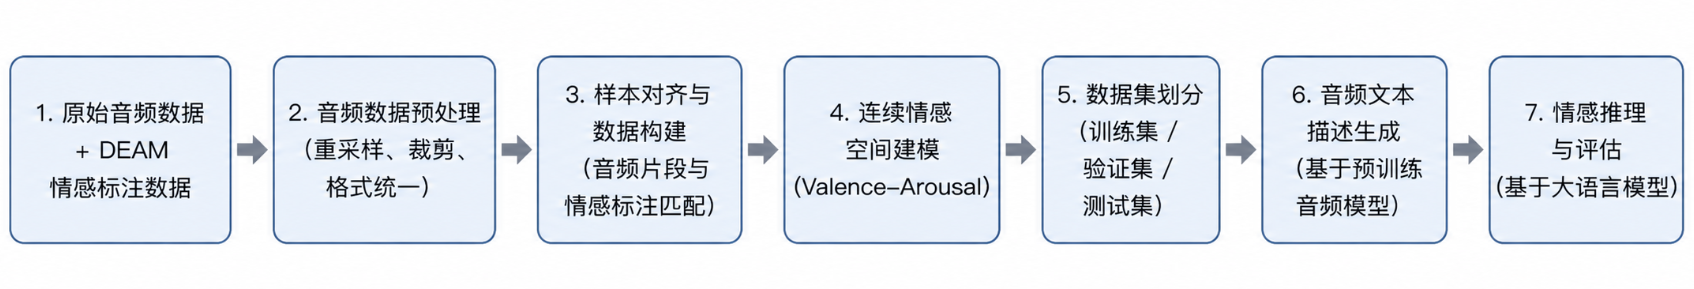
\includegraphics[width=1.0\linewidth]{image1.png}
    \caption{数据集划分流程}
    \label{fig:placeholder}
\end{figure}

\subsection{本章小结}
本章围绕系统的数据基础部分展开，介绍了本文所使用的 DEAM 数据集、情感标注体系以及音频数据预处理与数据集划分方法。首先，本文选择 DEAM 作为研究数据来源，并以 Valence-Arousal 二维情感模型作为主要情感表示方式。其次，通过音频预处理模块实现了原始音频的格式统一、重采样、单声道转换、静音裁剪和归一化处理，并构建了片段级元数据文件。最后，基于 Valence 和 Arousal 的分层抽样策略，系统完成了训练集、验证集和测试集的划分，为后续的音频描述生成、情感推理和对比实验提供了统一的数据基础。

从整体上看，本章所完成的数据集构建与预处理工作，为后续方法模块的实现提供了稳定的输入条件，也保证了实验过程具有一定的规范性与可复现性。下一章将在此基础上，进一步介绍基于预训练音频理解模型的音乐音频描述生成方法。

\newpage

\section{音频到文本描述生成方法}

\subsection{预训练音频理解模型调研与选型}

音乐音频描述生成任务的核心难点在于，系统不仅需要从音频信号中感知声音事件，还需要进一步理解音乐中的旋律走向、节奏形态、主要音色、曲风属性以及整体听感，并将这些信息组织为自然语言。与语音识别任务相比，音乐音频通常缺少明确的词边界，其情绪、风格和氛围等高层语义也具有较强的主观性。因此，本文所需的模型不仅要具备音频输入能力，还需要具有一定的跨模态理解能力和指令跟随能力。

从现有研究与工程实践来看，可用于音频处理的模型大体可分为三类：语音识别模型、音频特征或分类模型，以及多模态音频大模型。语音识别模型主要面向人声转写任务，适用于语音内容提取，但难以处理纯音乐或复杂器乐片段；音频特征与分类模型能够提取声学表示或输出固定类别，但通常不能直接生成结构化自然语言描述；多模态音频大模型则能够在音频输入基础上结合文本指令完成问答、摘要和内容描述，更符合本文“音频到文本描述”的任务需求。

为更加系统地比较不同模型在音乐音频描述任务中的适用性，本文选取若干具有代表性的模型进行横向分析，如表~\ref{tab:audio-models} 所示。

\begin{table}[htbp]
  \centering
  \caption{主流音频理解模型能力对比}
  \label{tab:audio-models}
  \begin{tabular}{lcccc}
    \hline
    模型 & 音频输入 & 指令跟随 & 描述生成 & 中文支持 \\
    \hline
    Whisper（语音识别） & 支持（语音） & 不支持 & 不支持 & 一般 \\
    VGGish / OpenL3（特征模型） & 支持 & 不支持 & 不支持 & 无关 \\
    AudioCLIP（跨模态模型） & 支持 & 部分支持 & 不支持 & 一般 \\
    SALMONN（音频大模型） & 支持 & 支持 & 支持 & 较弱 \\
    Qwen2-Audio-Instruct（音频大模型） & 支持 & 支持 & 支持 & 强 \\
    \hline
  \end{tabular}
\end{table}

由表~\ref{tab:audio-models} 可见，传统语音识别模型主要面向语音转写任务，缺乏对音乐语义的建模能力；音频特征模型虽然能够提供有效的数值表示，但难以直接输出可用于下游推理的自然语言描述；跨模态匹配模型更侧重于相似度计算或检索任务，而非开放式文本生成。相比之下，音频大模型在音频理解、文本生成和指令跟随方面具有更好的综合能力。

在候选模型中，Qwen2-Audio-Instruct 在中文生成、指令遵循和工程可用性方面较为均衡。该模型支持在输入音频的同时接收文本指令，能够根据给定约束生成特定格式的描述文本；同时，其中文输出质量较好，便于直接用于本文的实验展示和结果分析。因此，本文选择 Qwen2-Audio-Instruct 作为音频描述生成阶段的核心模型，并在此基础上通过输入预处理、提示词约束和质量检查等方法提升输出稳定性。

需要说明的是，本文并不对音频理解模型进行微调，而是以现有预训练模型为基础构建应用型实验流程。研究重点在于：通过合理的数据组织、音频输入处理和 Prompt 设计，使模型输出更加贴近音乐情感分析任务的需要。

\subsection{云端模型调用实现}

在模型选定之后，系统需要解决的关键问题是如何将本地音乐音频整理为接口可接收的输入形式，并稳定地批量生成描述结果。当前实现中，音频描述生成流程包括配置读取、测试样本加载、音频裁剪与编码、接口请求构造、响应解析以及结果保存等步骤。

首先，系统通过配置文件统一管理模型名称、服务提供方、接口地址、温度参数、最大输出长度、音频裁剪时长和样本数量上限等参数。采用配置文件而非脚本硬编码，有助于后续在不同实验设置之间快速切换。例如，当前音频裁剪时长设为 30 秒，系统在调用模型时优先使用每段音乐的前 30 秒内容；当 \texttt{max\_samples} 设置为 \texttt{null} 时，系统会对测试描述清单中的全部样本进行处理。本文后续实验使用与情感推理和传统基线对齐的 181 条测试样本，以保证不同方法之间的比较具有一致样本基础。

其次，描述生成模块以测试集样本清单作为输入。该文件包含样本编号、处理后音频路径以及对应的 Valence 和 Arousal 标注信息，因此系统能够逐条读取测试音频，并在输出描述时保留其真实情感标注。当前实现将测试集作为正式描述生成对象，训练集和验证集不在该阶段全量送入音频大模型，以控制接口调用成本，并使计算资源集中用于最终评估所需的样本子集。

在音频输入处理阶段，系统并未直接上传预处理后的 wav 文件，而是进一步进行接口适配。具体而言，系统将音频重新加载为 16 kHz 单声道波形，并对超过指定时长的片段截取前 30 秒内容。这一设计一方面能够降低请求体积，提升接口兼容性；另一方面也能减少超时和单次请求过长带来的不稳定因素。虽然只使用前 30 秒可能无法覆盖完整音乐结构，但多数片段开头已经包含较明显的旋律、节奏和配器信息，能够为描述生成提供基本依据。

在完成裁剪与重采样后，系统将音频编码为 base64 形式，并组装为可直接放入请求体的数据结构。该方式避免了额外文件上传流程，使本地音频能够以内嵌数据形式参与云端推理。接口调用时，系统采用“音频 + 文本指令”的联合输入方式，将音频内容与描述生成 Prompt 一并发送给模型。模型返回后，程序从响应中提取描述文本；若遇到请求超时、状态码异常或响应结构异常，则记录对应错误信息，而不直接中断整个批处理过程。

在结果保存方面，系统为每个测试样本记录样本编号、音频路径、真实 Valence 与 Arousal、生成描述及相关状态信息，并将结果写入表格文件。该结构化保存方式便于后续进行描述质量评估、情感推理和误差案例分析，也使音频描述结果能够与传统基线在同一样本维度上对齐。

\subsection{描述生成 Prompt 设计与多维度约束}

在基于音频大模型完成音乐描述生成的过程中，Prompt 设计直接影响输出内容的稳定性和下游可用性。若采用开放式描述请求，模型容易生成过于笼统的文本，或者将音乐联想到旅行、电影、人物和剧情等缺乏听觉依据的场景。为降低这类偏差，本文将描述生成 Prompt 设计为面向下游情感推理的结构化约束模板。

本文将描述生成约束划分为任务约束、内容维度约束、格式约束和表达风格约束四类，如表~\ref{tab:prompt-constraints} 所示。

\begin{table}[htbp]
  \centering
  \caption{描述生成 Prompt 约束设计}
  \label{tab:prompt-constraints}
  \begin{tabular}{ll}
    \hline
    约束类型 & 设计内容 \\
    \hline
    任务约束 & 仅基于音频内容生成描述，禁止无依据扩展 \\
    内容约束 & 覆盖旋律、节奏、乐器、曲风、整体听感五个维度 \\
    格式约束 & 单段文本，约 80--130 字，使用分号分隔五个分句 \\
    风格约束 & 使用保守表达，避免主观臆测、场景虚构和默认正向化 \\
    \hline
  \end{tabular}
\end{table}

在内容维度方面，系统要求模型依次描述旋律、节奏、乐器、曲风和整体听感。其中，旋律用于刻画音高走向、明暗倾向和句幅宽窄；节奏用于描述速度、疏密和律动强弱；乐器用于识别主要音色和频段分布；曲风用于给出保守的风格判断；整体听感则要求明确给出情绪档位与能量档位。该设计使文本描述不只停留在“好听”“轻快”等评价词层面，而是尽量覆盖可支撑情感推理的音乐要素。

本文在实验过程中对音频描述 Prompt 进行了两轮主要迭代。第一版 Prompt 已经固定“五句结构”，要求输出由分号分隔的五个分句，并在最后一个分句中明确给出情绪档位和能量档位。该版本的重点是将开放描述任务转化为结构化描述任务，同时明确禁止编造地名、旅行、电影、剧情和人物等内容。针对早期实验中常见的“默认写成轻快、跳跃、阳光明媚”的问题，第一版还加入了反偏置规则：当听感实际偏慢、偏暗、弱力度或低频较重时，禁止使用“轻盈”“活泼”“阳光”等正向模板词，除非音频中确有相应听觉依据。

第二版 Prompt 在第一版基础上进一步压缩语言风格，形成“白描精简体”。该版本将总字数收紧至约 80--130 字，要求输出恰好五个分句，并减少形容词堆叠。其核心目标是让描述更接近听觉事实：若音频表现为慢速、留白大或能量弱，文本中就应直接写出“慢”“留白大”“能量低”等信息，而不是为了语言流畅而写成“轻快”“跳跃”。同时，第二版继续保留第五句的情绪档位和能量档位约束，使上游描述能够为下游 Valence-Arousal 推理提供更明确的语义锚点。

表~\ref{tab:audio-prompt-iter} 概括了两版音频描述 Prompt 的主要差异。

\begin{table}[htbp]
  \centering
  \caption{音频描述 Prompt 迭代对比}
  \label{tab:audio-prompt-iter}
  \begin{tabular}{p{0.16\linewidth}p{0.36\linewidth}p{0.36\linewidth}}
    \hline
    版本 & 主要设计 & 解决的问题 \\
    \hline
    audio v1 & 固定五句结构；覆盖五个音乐维度；第 5 句明确情绪与能量 & 将自由描述转化为面向情感推理的结构化描述 \\
    audio v2 & 压缩字数；减少修辞；强化“慢、暗、弱力度”与“欢快、高能量”的区分 & 抑制描述默认正向化，降低上游文本对下游推理的误导 \\
    \hline
  \end{tabular}
\end{table}

从方法角度看，音频描述 Prompt 的优化重点不在于提高文本修辞性，而在于降低描述偏差和提升下游可用性。通过五维结构约束、情绪与能量显式标注，以及对默认正向词的限制，系统能够生成更稳定、更适合后续情感推理的音乐描述文本。

\subsection{描述质量评估与抽检方案}

音乐描述生成结果是否有效，不能仅以“成功返回文本”作为标准。对于后续情感推理任务而言，描述不仅需要语言通顺，还应尽可能覆盖关键音乐要素，减少明显幻觉，并在格式上保持稳定。因此，在完成描述生成之后，本文进一步设计了基于规则的描述质量评估模块，对生成结果进行自动筛查。

该评估方法不依赖额外训练模型，而是通过关键词匹配、长度统计和风险词检测等规则对描述文本进行分析。首先，系统构建旋律、节奏、乐器、曲风和整体听感五类关键词集合，并据此判断描述是否覆盖各音乐维度。其次，系统检查描述长度是否落在合理区间内，以发现信息过少或输出过长的问题。再次，系统检测保守性措辞和幻觉风险词，例如“可能”“偏向”“疑似”等词用于观察不确定性表达，而“夏威夷”“电影画面”“人物”“故事情节”等词则用于识别可能超出音频依据的场景化联想。

在综合评分上，系统将维度覆盖、长度合理性和风险控制情况汇总为质量分数，并划分为 PASS、WARN 和 FAIL 三类。该方法属于启发式自动评估，不能完全替代人工听评，但能够快速发现格式异常和明显偏离任务要求的输出，适合作为批量实验中的初步筛查手段。

从当前实验结果来看，在与情感推理和基线评估一致的 181 条有效测试样本上，描述质量评估结果为 PASS 177 条、WARN 4 条、FAIL 0 条，平均得分为 95.03。结果如表~\ref{tab:desc-quality} 所示。

\begin{table}[htbp]
  \centering
  \caption{描述生成质量规则评估结果}
  \label{tab:desc-quality}
  \begin{tabular}{lcc}
    \hline
    指标 & 数量 & 占比（\%） \\
    \hline
    PASS & 177 & 97.79 \\
    WARN & 4 & 2.21 \\
    FAIL & 0 & 0.00 \\
    \hline
    平均得分 & \multicolumn{2}{c}{95.03} \\
    \hline
  \end{tabular}
\end{table}

上述结果表明，在当前音频输入处理和 Prompt 约束下，大多数描述能够满足长度、结构和维度覆盖要求。对于少量 WARN 样本，仍需要结合原始音频进行人工复核，以区分“表达不够充分”和“语义偏差明显”等不同情况。由于规则法主要依赖表层特征，难以完全判断描述是否与真实听感一致，因此后续可通过人工抽检进一步补充评价，例如从准确性、完整性、自然性和幻觉风险四个维度对部分样本进行评分。

\subsection{本章小结}

本章围绕音乐音频到文本描述生成任务，介绍了模型选型、云端调用、Prompt 设计与描述质量评估方法。本文选择 Qwen2-Audio-Instruct 作为核心音频理解模型，并通过统一配置、音频裁剪、重采样、base64 编码和批量落盘等步骤构建描述生成流程。在 Prompt 设计方面，本文从结构化描述、反场景幻觉和反默认正向偏置三个角度进行优化，并通过两版音频 Prompt 的迭代提升描述对下游情感推理的适配性。实验结果表明，在 181 条测试样本上，生成描述整体质量较为稳定，可作为后续大语言模型情感推理的输入基础。

\newpage

\section{基于大语言模型的情感推理方法}

\subsection{情感推理任务建模}

在上一章中，本文完成了从音乐音频到自然语言描述的转换。通过引入音频描述这一中间语义层，原本难以直接解释的音频信号被转化为包含旋律、节奏、乐器、曲风和整体听感等信息的文本表示。在此基础上，本文将音乐情感识别进一步建模为基于文本语义的推理任务。

具体而言，系统首先读取音频描述文本，然后构造面向情感分析的 Prompt，引导大语言模型输出音乐片段在 Valence 与 Arousal 两个连续维度上的预测值。设原始音频为 $x$，音频描述模型为 $g(\cdot)$，情感推理模型为 $f(\cdot)$，则两阶段过程可表示为
\begin{equation}
\begin{aligned}
d &= g(x), \\
(v,a) &= f(d),
\end{aligned}
\end{equation}
其中，$d$ 表示音频描述文本，$v$ 表示 Valence，$a$ 表示 Arousal。随后，系统通过统一映射函数 $h(\cdot)$ 将连续情感维度映射为离散标签：
\begin{equation}
l=h(v,a).
\end{equation}

本文采用“连续值预测 + 离散标签映射”的双层表示方式。一方面，Valence 和 Arousal 能够与 DEAM 数据集的原始连续标注直接对齐，便于计算 MAE、RMSE 和 Pearson 相关系数；另一方面，离散标签更便于展示和分类分析。为了保证大语言模型方法与传统基线方法在标签层面的可比性，本文不再让大语言模型直接输出标签，而是统一由映射函数 $h$ 根据 $(v,a)$ 生成标签。

该任务建模方式具有两个优点。首先，它将复杂的音频情感识别拆解为“音频语义描述”和“文本情感推理”两个阶段，使误差来源更容易分析。其次，文本描述作为中间结果具有可读性，能够帮助研究者判断模型是否正确捕捉到音乐要素，以及后续情感推理是否受到描述偏差影响。

\subsection{LLM 模型选型与 API 实现}

在情感推理阶段，本文采用云端大语言模型接口完成批量推理。该方案与音频描述生成阶段保持一致，能够降低本地部署和模型训练成本，使研究重点集中在任务建模、Prompt 设计和实验分析上。

在模型选型过程中，本文对国际主流模型、国内主流模型和开源模型进行了比较，如表~\ref{tab:llm-survey} 所示。比较维度包括中文语义理解、推理能力、输出一致性和工程可用性。

\begin{table}[htbp]
  \centering
  \caption{情感推理阶段大语言模型调研对比}
  \label{tab:llm-survey}
  \resizebox{\linewidth}{!}{
  \begin{tabular}{lccccc}
    \hline
    模型类别 & 代表模型 & 中文语义理解 & 推理能力 & 输出一致性 & 工程可用性 \\
    \hline
    国际主流模型 & GPT-4 系列 / Claude 3 等 & 很强 & 很强 & 很高 & 较高（成本较高） \\
    国内主流模型 & Qwen-Plus / GLM-4 / ERNIE Bot & 很强 & 强 & 高 & 高（成本可控） \\
    开源模型 & LLaMA 3 / Mistral & 较强 & 较强 & 中等 & 一般（需自行部署） \\
    \hline
  \end{tabular}
  }
\end{table}

从任务需求看，情感推理阶段的输入是中文音乐描述文本，其中包含旋律、节奏、乐器、曲风和整体听感等多维语义线索。模型需要综合这些文本信息，将其映射到 DEAM 的 1--9 连续量表。该任务需要一定的语义理解和上下文综合能力，但并不依赖极端复杂的长链推理。因此，在模型选型时，除推理能力外，还需要考虑接口稳定性、中文支持、调用成本和批量实验可操作性。

综合比较后，本文选用 Qwen-Plus 作为情感推理阶段的核心模型。该模型在中文语义理解、结构化输出和接口可用性方面较为均衡，能够支持 181 条测试样本及多轮 Prompt 版本的批量推理。系统在实现上采用配置驱动方式管理模型名称、接口地址、温度参数和最大输出长度等信息，使不同模型或不同 Prompt 版本之间的切换更加方便。

需要说明的是，本文并不以训练或微调大语言模型为目标，而是关注“音频描述生成—情感推理”这一方法链路的有效性。因此，在模型能力满足任务要求的前提下，工程可行性和实验成本控制是本文模型选型的重要依据。

\subsection{提示词模板设计与迭代优化}

大语言模型具有较强的开放式生成能力。若缺少明确约束，模型可能输出解释性文字、Markdown 代码块、额外字段，或者给出与量表含义不一致的数值。为提升输出稳定性，本文采用“角色设定 + 量表说明 + 输出格式约束”的 Prompt 设计方式，并在实验过程中进行了多轮迭代。

情感推理 Prompt 由 system prompt 和 user prompt 两部分组成。system prompt 用于设定模型角色、解释 Valence-Arousal 标度，并约束输出字段；user prompt 用于插入具体音乐描述，并再次强调 JSON 输出格式。整个设计目标是使模型只输出可被程序稳定解析的 \texttt{valence} 与 \texttt{arousal} 两个字段，并将离散标签交由下游统一映射。

本文共形成 v1 至 v5 五个情感推理 Prompt 版本，其中 v2 属于加入标签联合输出的中间探索版本，主实验主要对 v1、v3、v4 和 v5 进行了完整评估。各版本的核心变化如表~\ref{tab:llm-prompt-iter} 所示。

\begin{table}[htbp]
  \centering
  \caption{情感推理 Prompt 迭代过程}
  \label{tab:llm-prompt-iter}
  \begin{tabular}{p{0.12\linewidth}p{0.43\linewidth}p{0.35\linewidth}}
    \hline
    版本 & 主要变化 & 目的 \\
    \hline
    v1 & 仅要求根据描述输出 Valence 与 Arousal 两个 JSON 字段 & 打通基础推理与解析流程 \\
    v2 & 加入 1--9 量表说明，并尝试同时输出离散标签 & 提升量表理解，探索联合输出可行性 \\
    v3 & 移除 label 字段，规定标签由系统下游统一映射 & 降低多任务干扰，保证与基线口径一致 \\
    v4 & 强化中性区间、反高效价偏置和反塌缩约束 & 修正“好听/丰富/层次感”导致的 Valence 虚高 \\
    v5 & 进一步强调只依据文本线索，并要求拉开相邻样本微差 & 尝试提升连续量表分辨率 \\
    \hline
  \end{tabular}
\end{table}

从迭代逻辑看，v1 版本主要用于验证模型能否稳定输出两维 JSON，但缺少对量表含义的解释，容易出现数值使用不稳定的问题。v2 在此基础上加入 Valence 和 Arousal 的区间说明，并尝试让模型同时输出离散标签，但实验中发现数值与标签可能存在不一致。v3 因此取消 label 字段，改为只输出连续值，再由映射函数 $h$ 统一生成标签，从而减少自由文本标签带来的额外噪声。

后续实验发现，大语言模型容易将“温暖”“丰富”“层次感强”等描述理解为高愉悦度，导致 Valence 系统性偏高。针对这一问题，v4 明确规定：当描述主要表现为中性、氛围、铺陈或器乐化特征，且缺少明确欢快、明亮、节庆感等积极情绪线索时，Valence 应优先落在 4--6.5 区间；同时强调 Valence 与 Arousal 可以独立判断，不必同时升高。v4 还加入“反塌缩”约束，要求模型避免大量样本重复使用完全相同的少数刻度。

v5 在 v4 基础上进一步强化“只依据描述中实际出现的线索”和“避免机械重复同一对数值”的要求。但从实验结果看，v5 的约束更强，并未带来最优指标，说明 Prompt 约束并非越多越好，过强的限制可能反而影响模型对真实情绪线索的综合判断。因此，本文在结果分析中将 v4 视为本轮情感推理 Prompt 迭代中的最佳版本，并与传统基线进行重点比较。

\subsection{批量推理流程与结果解析实现}

在单条样本推理可以正常进行的基础上，系统还需要支持多样本批量推理、结果解析、异常处理和断点续跑。情感推理模块首先读取真实音频生成的描述文件；若真实描述文件不存在，则可回退到占位描述文件，用于开发阶段快速打通流程。正式实验中，系统使用 181 条真实测试描述作为输入。

在正式推理过程中，系统逐行读取描述文本，将其填入 user prompt 中，并结合对应版本的 system prompt 构造请求消息。模型返回后，系统保留原始响应文本，同时通过 JSON 提取逻辑解析 \texttt{valence} 和 \texttt{arousal} 字段。若模型响应中包含额外文本，解析函数会尝试提取第一个合法 JSON 对象；若仍无法解析，则该样本被记录为无效预测，以便后续评估时跳过或统计。

为提高长时间批量实验的稳定性，系统实现了断点续跑和分批落盘机制。当输出文件已存在时，系统会读取已完成样本编号并跳过重复样本，避免因中途异常而重新调用已完成请求；同时，系统在处理一定数量样本后将结果写入文件，以减少运行中断造成的数据损失。最终结果文件记录样本编号、描述文本、真实情感标注、预测 Valence、预测 Arousal、模型原始输出、推理耗时和 Prompt 版本等信息，为后续指标计算和案例分析提供数据基础。

\subsection{情感标签生成与映射策略}

在本研究中，离散情感标签并不由大语言模型直接生成，而是通过统一映射函数 $h$ 由连续情感维度得到。具体而言，大语言模型首先基于描述文本预测 $(v,a)$，随后系统计算：
\begin{equation}
l = h(v,a),
\end{equation}
其中，$l$ 为离散情感标签。真实标签同样由数据集中给出的 $(v_{\mathrm{true}},a_{\mathrm{true}})$ 经过统一的映射函数生成，从而保证大语言模型路径与回归基线及分类基线在标签评价过程中采用一致的评价口径，提高结果之间的可比性。

早期实验曾尝试让大语言模型直接输出 label 字段，但该方式可能产生两类问题：一是模型输出的标签与其给出的 Valence-Arousal 数值不一致；二是自由标签会引入额外的类别定义差异，降低与传统基线的可比性。因此，最终主实验采用“连续值预测 + 统一映射”的策略。该策略更符合 DEAM 数据集以连续标注为主的特点，也使分类结果能够与连续预测误差关联分析。

需要指出的是，映射函数虽然增强了结果可解释性，但也会放大边界附近的连续误差。例如，当某个样本的真实值与预测值只存在较小数值差异，但刚好跨过阈值边界时，离散标签可能发生变化，从而在分类准确率上表现为错误。因此，本文在第五章中同时报告连续指标和离散准确率，避免仅依赖单一指标评价模型性能。

\subsection{本章小结}

本章介绍了基于大语言模型的情感推理方法。本文将音乐情感识别建模为基于描述文本的连续情感维度预测任务，并通过统一映射函数获得离散标签。在模型实现方面，系统采用 Qwen-Plus 云端接口完成批量推理，并通过配置文件管理模型与 Prompt 版本。在 Prompt 设计方面，本文经历了从基础 JSON 输出、量表说明、移除 label 字段，到反高效价偏置和反塌缩约束的多轮迭代。实验设计上，最终采用统一的 $(v,a)\rightarrow l$ 映射口径，为第五章同样本对比传统基线奠定基础。

\newpage

\section{对比实验与结果分析}

\subsection{实验设置与评价指标}

为在统一数据划分和可复现流程下比较不同方法，本文将实验设计为三个相互衔接的环节：音乐音频描述生成、基于描述文本的 Valence-Arousal 预测，以及基于传统声学特征的机器学习基线。各环节通过统一配置管理参数，并在相同测试子集上进行评估，以保证结果具有可比性。

实验程序基于 Python 实现，涉及音频处理、数据分析、模型接口调用和机器学习建模等工具。描述生成阶段调用 Qwen2-Audio-Instruct 生成中文音乐描述；情感推理阶段调用 Qwen-Plus，根据描述文本输出 Valence 与 Arousal；传统基线则以声学特征为输入，分别训练 Ridge 回归模型和 Logistic Regression 分类模型。

在数据划分方面，传统基线使用全部可用训练样本进行模型拟合，共 1260 条；测试阶段选取同时具备完整声学特征与文本描述的样本子集，共 181 条。大语言模型方法和传统基线均在这 181 条样本上进行评估，离散标签均由同一映射函数 $h$ 得到。这样可以避免因测试样本不一致或标签定义不同导致的比较偏差。

评价指标分为三个层面。对于描述文本，采用规则法统计 PASS、WARN、FAIL 和平均质量得分；对于连续情感维度，采用平均绝对误差（MAE）、均方根误差（RMSE）和 Pearson 相关系数 $r$；对于离散情感标签，采用分类准确率。设第 $i$ 个样本的真实值为 $y_i$，预测值为 $\hat{y}_i$，样本量为 $n$，则：
\begin{equation}
\mathrm{MAE}=\frac{1}{n}\sum_{i=1}^{n}|y_i-\hat{y}_i|,
\end{equation}
\begin{equation}
\mathrm{RMSE}=\sqrt{\frac{1}{n}\sum_{i=1}^{n}(y_i-\hat{y}_i)^2}.
\end{equation}
分类准确率定义为：
\begin{equation}
\mathrm{Accuracy}=\frac{\text{正确分类样本数}}{\text{总样本数}}.
\end{equation}
其中，MAE 和 RMSE 越低表示误差越小，Pearson 相关系数越高表示预测值与真实值变化趋势越一致。

\subsection{LLM 情感推理与 Prompt 迭代结果分析}

本文首先对不同情感推理 Prompt 版本进行比较，以观察提示词设计对大语言模型结果的影响。表~\ref{tab:prompt-results} 汇总了主要运行版本在 181 条测试样本上的评估结果。由于 v2 属于中间探索版本，主要用于验证 label 联合输出的可行性，未作为最终主表运行版本；因此表中列出 v1、v3、v4 和 v5 的结果。

\begin{table}[htbp]
  \centering
  \caption{不同情感推理 Prompt 版本的评估结果（$n=181$）}
  \label{tab:prompt-results}
  \resizebox{\linewidth}{!}{
  \begin{tabular}{lccccc}
    \hline
    版本 & Valence MAE & Valence $r$ & Arousal MAE & Arousal $r$ & 标签准确率 \\
    \hline
    v1 & 2.251 & 0.222 & 1.612 & 0.559 & 0.138 \\
    v3 & 2.136 & 0.266 & 1.651 & 0.548 & 0.177 \\
    v4 & 1.652 & 0.348 & 1.393 & 0.494 & 0.309 \\
    v5 & 1.966 & 0.307 & 1.712 & 0.544 & 0.160 \\
    \hline
  \end{tabular}
  }
\end{table}

从表~\ref{tab:prompt-results} 可以看出，v1 作为基础版本能够完成结构化输出，但在 Valence 误差和标签准确率方面表现较弱。v3 通过移除 label 字段、统一由系统映射标签，略微提升了标签准确率，并降低了输出不一致风险。v4 的提升最明显：Valence MAE 从 v3 的 2.136 降至 1.652，Arousal MAE 从 1.651 降至 1.393，标签准确率提升至 0.309。说明针对高效价偏置、中性区间和输出塌缩问题的 Prompt 约束能够有效改善模型预测结果。v5 虽进一步强化了反偏置和反重复约束，但整体表现反而下降，表明过强或过细的限制可能削弱模型对整体语义的综合判断。

从误差机制看，v4 的主要价值在于明确区分“制作质量词”和“情绪效价词”。早期版本中，模型容易将“温暖、丰富、有层次、细腻”等描述理解为高愉悦度，从而导致 Valence 虚高。v4 明确规定：当文本主要表现为氛围、铺陈、器乐化或配器细节，且缺少明确欢快、明亮、强积极情绪线索时，Valence 应优先落入中性区间。这一约束使模型在面对中性或弱情绪文本时更加保守，从而显著降低了效价误差。

结合音频描述 Prompt 的两轮迭代可以看出，系统性能提升并非来自单一阶段，而是来自上游描述偏差抑制和下游量表推理校准的共同作用。音频描述 Prompt 通过反默认正向化规则减少输入文本偏差；情感推理 Prompt v4 则进一步抑制 LLM 对正向词和华丽修辞的过度响应。二者共同使两阶段大模型路径在标签准确率上明显缩小了与 Ridge 回归后映射基线的差距。

\subsection{与传统声学特征基线的对比}

为评价两阶段大模型方法的相对表现，本文构建了基于传统声学特征的机器学习基线。该基线以预提取的时序声学特征为输入，对每个片段的特征列计算均值、标准差、最小值、最大值与中位数，并拼接为 1305 维片段级特征向量。连续情感预测采用 Ridge 回归模型，离散情感分类采用带类别权重的 Logistic Regression 模型。特征在进入模型前进行标准化处理，以降低不同特征量纲差异的影响。

基线模型使用 1260 条训练样本进行拟合，并在与 LLM 方法相同的 181 条测试样本上评估。连续指标对比如表~\ref{tab:main-metrics} 所示，离散标签准确率如表~\ref{tab:label-acc} 所示。为体现 Prompt 迭代后的最佳大模型结果，表中采用 v4 作为 LLM 代表版本。

\begin{table}[htbp]
  \centering
  \footnotesize
  \caption{连续情感维度预测结果对比（$n=181$；RMSE 与 MAE、$r$ 同源汇总文件）}
  \label{tab:main-metrics}
  \begin{tabular}{lcccccc}
    \hline
    方法 & 效价 MAE & 效价 RMSE & 效价 $r$ & 唤醒 MAE & 唤醒 RMSE & 唤醒 $r$ \\
    \hline
    两阶段 LLM（v4） & 1.652 & 1.927 & 0.348 & 1.393 & 1.741 & 0.494 \\
    声学特征 + Ridge 基线 & 1.014 & 1.307 & 0.512 & 0.976 & 1.267 & 0.605 \\
    \hline
  \end{tabular}
\end{table}

\begin{table}[htbp]
  \centering
  \caption{离散情感标签准确率对比（统一映射 $h$，$n=181$）}
  \label{tab:label-acc}
  \begin{tabular}{lc}
    \hline
    方法 & 准确率 \\
    \hline
    两阶段 LLM（v4，经 $h$ 映射） & 0.309 \\
    基线：Ridge 回归后映射 & 0.354 \\
    基线：LogReg 直接多分类 & 0.381 \\
    \hline
  \end{tabular}
\end{table}

\begin{figure}
    \centering
    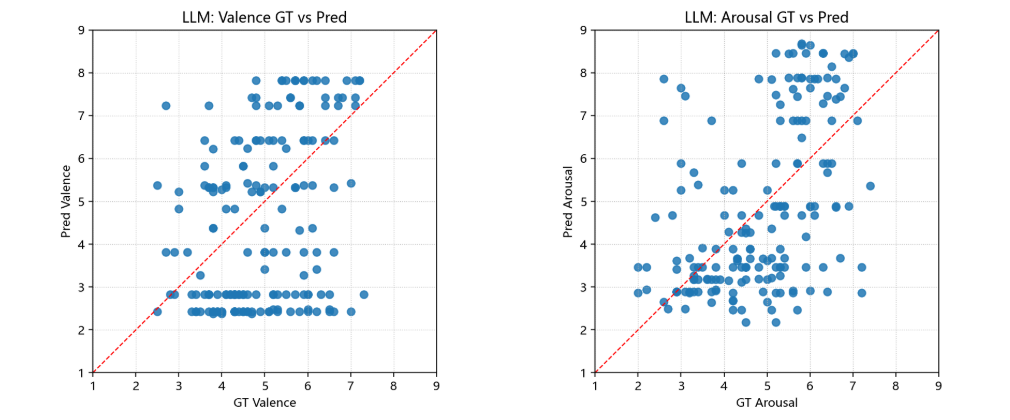
\includegraphics[width=1.0\linewidth]{image2.png}
    \caption{两阶段 LLM（v4）在 Valence 与 Arousal 维度上的真值--预测散点图}
    \label{fig:placeholder}
\end{figure}

\begin{figure}
    \centering
    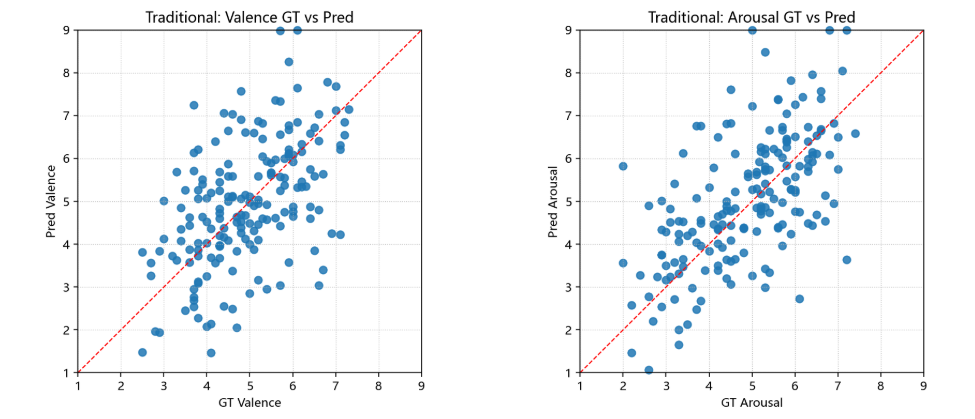
\includegraphics[width=1.0\linewidth]{image3.png}
    \caption{传统声学特征基线在 Valence 与 Arousal 维度上的真值--预测散点图}
    \label{fig:placeholder}
\end{figure}

由表~\ref{tab:main-metrics} 可见，传统声学特征基线在连续情感预测方面仍具有更低误差和更高相关性。图~\ref{fig:llm-v4-scatter} 与图~\ref{fig:baseline-scatter} 进一步展示了两类方法在连续空间中的拟合差异：LLM 路径经过 v4 提示词校正后，预测分布较早期版本更加接近真实标注，但仍可观察到一定的中间区间聚集；传统基线的预测点云整体更接近理想对角线。其原因在于基线模型直接以 DEAM 标注作为监督目标进行拟合，而大语言模型路径需要经历“音频到文本描述”和“文本到情感维度”两个阶段，误差可能在链式过程中累积。尤其在 Valence 维度上，大语言模型对细粒度愉悦度标度的把握仍弱于监督回归模型。

从离散标签准确率看，LLM v4 的准确率达到 0.309，与 Ridge 回归后映射的 0.354 相比差距已缩小，但仍低于 LogReg 直接分类的 0.381。这说明经过 Prompt 迭代后，大语言模型方法在类别层面有所进步，但尚未超过传统监督学习方法。相比早期 v1 的 0.138，v4 的提升幅度较明显，表明提示词迭代对两阶段方法具有实质性改进作用。

需要指出的是，传统基线和大模型方法的优势并不完全相同。传统基线在当前标注空间中直接学习，量化指标更稳定；大模型方法虽然数值指标略弱，但能够输出可阅读的中间描述，使研究者可以进一步分析“模型听到了什么”和“为什么会做出该情感判断”。因此，本文并不将两阶段大模型方法简单定位为传统基线的替代，而是将其作为一种具有可解释中间层的音乐情感分析路径。

\subsection{两类方法对比与优劣分析}

在同样本、同量表和同一标签映射函数 $h$ 的条件下，本文对两阶段 LLM 方法和传统声学特征基线进行了对比。总体来看，传统基线在连续值预测和离散标签准确率上仍占优；而两阶段 LLM 方法的主要优势在于语义解释能力、流程可分析性和 Prompt 可迭代性。

从预测效果看，声学特征基线直接利用训练集标注进行监督学习，目标函数与评价指标一致，因此能够较稳定地拟合 Valence 和 Arousal。两阶段 LLM 方法没有在 DEAM 标注上进行参数训练，其输出依赖上游描述质量和下游文本推理能力，因此在细粒度标度对齐方面更容易出现偏差。特别是 Valence 维度，文本中的“温暖”“细腻”“丰富”等词容易被模型误读为强正向情绪，导致预测值偏高。

从可解释性看，两阶段 LLM 方法具有传统基线不具备的中间文本表示。传统基线的输入是高维声学特征向量，虽然对回归和分类有效，但难以直观解释其情感判断依据；而 LLM 方法先生成音乐描述，再基于描述进行推理，研究者可以从描述文本中观察旋律、节奏、乐器和整体听感等线索。这为误差分析提供了更直接的入口。

从工程扩展性看，两类方法也体现出不同特点。传统基线依赖稳定的特征提取流程和监督学习模型，适合构建性能参照；大模型方法则可以通过更换音频理解模型、调整 audio prompt（音频侧提示词）、迭代情感推理 prompt 或引入校准策略继续优化。在本研究中，v4 prompt 已将 LLM 标签准确率明显提升，拉近了与 Ridge 回归后映射基线的差距，说明 Prompt 工程在不重新训练模型的条件下仍具有一定改进空间。

因此，本文的实验结论可以概括为：在当前数据和实验设置下，传统声学特征基线仍是量化指标更优的方法；经过 Prompt 迭代后的两阶段 LLM 方法虽未超过传统基线，但已经明显优于早期版本，并在语义可解释性方面具有补充价值。

\subsection{误差分析与系统不足}

实验误差可能来自音频描述生成、文本情感推理和标签映射三个环节。首先，上游描述并不总能完全等同于真实听感。即使描述质量规则评估为 PASS，文本也可能存在主观表达、维度偏弱或场景联想问题。例如，若描述中出现缺乏音频依据的画面化词汇，后续 LLM 可能依据这些语义进行情感推理，从而偏离真实标注。

其次，情感推理阶段仍存在标度对齐问题。大语言模型擅长根据文本判断情绪方向，但对 DEAM 量表中 1--9 的连续细分并不天然稳定。v4 通过中性区间约束和反高效价偏置显著改善了结果，但 Valence 误差仍高于传统基线，说明单纯依赖提示词仍难完全替代有监督回归模型。

第三，离散标签映射会放大边界附近误差。本文采用统一函数 $h$ 将连续值转换为六类标签，这有利于方法对比，但也意味着当预测值在阈值附近发生轻微偏移时，离散标签可能发生变化。因此，标签准确率应结合连续指标共同分析，而不宜单独作为系统性能的唯一依据。

第四，实验复现性仍有进一步完善空间。大模型侧已经能够从逐样本预测文件复现汇总指标和图表；但传统基线使用的声学特征若依赖外部提取流程，则仍需进一步补充特征生成脚本或说明特征来源。否则，读者难以从原始音频开始完全复现传统基线实验。

此外，描述质量评估目前主要依赖规则法，能够检查长度、维度覆盖和显性风险词，但难以全面判断文本与音频真实听感是否一致。后续若能加入人工抽检或专家评分，将有助于更准确地评估上游描述质量，并进一步分析描述质量与情感推理误差之间的关系。

综上，当前系统的不足主要包括：音频描述仍可能存在语义偏差；大语言模型对连续情感量表的精细对齐能力有限；离散映射对边界误差较敏感；传统特征链路的复现性仍需加强；描述质量缺少系统人工评估。这些不足并不否定两阶段方法的研究价值，而是指出了后续改进的具体方向。

\subsection{本章小结}

本章围绕实验设置、Prompt 迭代结果、传统基线对比和误差分析展开。实验结果表明，在 181 条同样本测试集上，情感推理 Prompt 从 v1 迭代至 v4 后，LLM 路径的标签准确率由 0.138 提升至 0.309，与传统 Ridge 回归后映射基线的 0.354 相比差距明显缩小，但仍低于 LogReg 分类基线的 0.381。在连续情感维度上，传统声学特征基线仍具有更低误差和更高相关性（见表~\ref{tab:main-metrics} 中的 MAE、RMSE 与 $r$）。总体而言，本文构建的两阶段大模型方法在量化指标上尚未超过传统基线，但通过 Prompt 迭代显著改善了初始结果，并在中间语义可解释性和流程可分析性方面体现出一定优势。

\newpage
\section{总结与展望}

\subsection{工作总结}

本文围绕“基于大语言模型的音乐音频信号描述与情感标签生成”这一课题，针对音乐情感分析任务中语义表达不足与结果可解释性有限的问题，设计并实现了一套两阶段音乐情感分析方法。该方法首先利用具备音频理解能力的多模态模型对音乐音频片段生成自然语言描述，再基于大语言模型对描述文本进行情感推理，输出对应的 Valence 与 Arousal 连续情感维度，并进一步映射为离散情感标签，从而构建起从原始音频到可解释情感结果的完整处理流程。

在数据准备方面，本文基于 DEAM 数据集构建实验数据基础。通过整合静态情感标注与原始音频数据，完成了样本筛选、音频预处理及数据组织等工作。具体包括音频重采样、单声道转换、静音裁剪与音量归一化等处理，并将音频数据与对应情感标注统一组织为结构化形式，为后续实验提供规范化输入。同时，采用基于 Valence 与 Arousal 分布的分层抽样方法完成数据集划分，提高了实验结果的稳定性与可复现性。

在音乐音频描述生成方面，本文基于预训练音频理解模型构建了自动化描述生成模块，实现了从音频输入到文本描述输出的处理流程。在提示词设计上，围绕旋律、节奏、乐器、曲风及整体听感等维度对生成内容进行约束，以提升描述的语义完整性。同时，引入基于规则的描述质量评估方法，从文本长度、要素覆盖与异常表述等方面对结果进行筛选，从而为后续情感推理提供相对稳定的输入。

在情感预测方面，大语言模型输出连续情感维度 $(v,a)$，离散情感标签通过与基线方法一致的映射函数 $h$ 由连续值生成，并与由真实标注经同一映射得到的参考标签进行统一比较，从而保证评价标准的一致性。

在实验与对比分析方面，本文构建了基于声学特征的传统基线方法，包括岭回归（Ridge）与逻辑回归（Logistic Regression）模型。在统一样本集合、统一情感量表及一致映射函数 $h$ 的条件下进行对比实验。实验结果表明，传统基线方法在连续情感预测指标（MAE、RMSE、Pearson 相关系数）以及离散情感分类准确率方面整体优于基于大语言模型的两阶段方法。

与此同时，基于大语言模型的方法在中间文本表示的可解释性、处理流程的分阶段分析能力以及提示词设计的可调节性方面表现出一定优势，为后续方法优化提供了新的研究视角。

总体而言，本文完成了从数据准备、音频描述生成、情感推理到基线构建与结果分析的系统性研究工作，构建并验证了一条完整且可复现的音乐情感分析流程，并在统一评价框架下对不同方法进行了对比分析，为后续研究与方法改进提供了基础。

此外，实验结果表明，两阶段方法在引入语义中间表示的同时，可能存在误差在多阶段过程中累积的问题，这为后续优化模型结构与提示词设计提供了进一步研究方向。

\subsection{主要成果与不足}
从当前课题的完成情况来看，已有工作在系统构建、实验验证与工程实现等方面取得了一定进展，主要体现在以下几个方面。

首先，完成了音乐情感分析任务的整体流程设计与实现。相较于仅依赖传统声学特征进行回归或分类的方法，所构建的方法引入音频描述作为中间语义表示，将复杂的音频信号转化为结构化文本信息，并在此基础上开展情感推理，形成“音频—文本描述—情感预测”的两阶段处理框架。

其次，完成了关键功能模块的工程化实现，包括音频预处理、描述生成、描述质量评估、大语言模型情感推理以及传统基线对比模块，系统具备从数据输入到结果输出的完整运行能力。

最后，在主实验设置下，已在 181 条测试样本上完成完整实验流程，并结合 1260 条训练样本构建传统基线模型，形成了可核对的实验结果记录与同样本对比分析。

为进一步对两类方法在不同维度上的表现进行系统归纳与对比分析，并从方法结构、性能表现及工程特性等方面进行综合评估，表 \ref{tab:method-comparison} 对两阶段大语言模型方法与传统声学特征基线方法的主要差异进行了整理与总结。

\begin{table}[htbp]
  \centering
  \caption{两类方法在音乐情感分析任务中的综合对比（基于主实验结果总结）}
  \label{tab:method-comparison}
  \begin{tabular}{p{0.25\linewidth}p{0.33\linewidth}p{0.35\linewidth}}
    \hline
    对比维度 & 两阶段大语言模型方法 & 传统声学特征基线方法 \\
    \hline
    方法结构 & 音频描述 + 文本推理 & 声学特征 + 监督学习 \\
    可解释性 & 较强（具备中间语义描述） & 较弱（特征语义有限） \\
    性能 & 相对较弱（连续与分类指标均低于基线） & 相对较强（主实验指标表现更优） \\
    工程实现复杂度 & 中等（多模块协同） & 中等（特征与模型训练） \\
    可复现性 & 较高（流程完整可复现） & 受特征提取流程影响 \\
    分析灵活性 & 较高（支持分阶段分析） & 较低（整体黑箱） \\
    \hline
  \end{tabular}
\end{table}

由表 \ref{tab:method-comparison} 可以看出，两阶段大语言模型方法在可解释性与分析灵活性方面具有一定优势，能够提供中间语义层用于分析与调试；而传统声学特征基线方法在连续情感预测精度与离散标签准确率方面整体表现更优，该结论与前文基于主实验指标的分析结果一致。

尽管已取得上述进展，当前工作仍存在一定不足。其一，在连续情感维度拟合与标签准确率方面，大语言模型路径整体性能仍低于传统基线；其二，部分声学特征依赖外部处理流程，当前仓库尚未完全覆盖从原始音频到特征生成的完整链路；其三，描述质量与情感预测效果主要依赖规则评估，缺乏系统人工评价；其四，主实验仍基于片段级静态标注，尚未引入时间动态建模。

综上，当前工作的主要成果在于构建了可运行的两阶段实验流程，并形成了可核对的实验结果记录与同样本对比分析；主要不足体现在模型性能仍有差距以及评价与复现体系有待进一步完善。其中，性能差异表明传统方法在当前数据规模与评价体系下仍具有优势，而两阶段方法的价值主要体现在中间语义表达与分析过程的可解释性。

\subsection{后续优化方向与展望}
结合当前实验结果与系统实现情况，后续工作可从以下几个方面进一步展开。

首先，在保持主实验划分与评价流程一致的前提下，可通过替换音频理解模型或文本大语言模型，或对现有提示词进行迭代优化，在相同数据划分与评估口径下重新报告表 \ref{tab:main-metrics} 与表 \ref{tab:label-acc}，以实现不同方案间的可比性分析。若扩展至更大规模数据，应明确说明样本规模与划分策略。

其次，在实验复现方面，大语言模型推理链路已基本具备自动化能力，而传统基线部分仍需进一步完善。后续应明确声学特征的来源，或将特征提取过程纳入统一代码仓库，以支持从原始音频到模型训练的全流程复现。

第三，在音频描述生成环节，仍存在维度覆盖不均、描述长度波动及语义外延偏移等问题。后续可通过细化提示词约束（如强制五维句式结构）、优化模型参数设置以及对比不同音频处理策略，进一步提升描述生成的一致性与稳定性。

第四，在情感推理阶段，可通过引入少样本提示、对比示例或后处理校准策略，在不依赖专门微调的前提下改善情感量表的对齐效果。不同提示策略需在统一评价口径下独立报告，避免结果混用。

第五，可引入人工评测与案例分析机制。通过构建小规模人工标注数据，从准确性、完整性与表达合理性等维度对描述质量进行评估，同时结合典型样本分析情感预测误差来源，以增强实验分析深度。

第六，可进一步探索动态情感建模方法。当前系统基于片段级平均情感值进行建模，未反映音乐情感的时间变化特性。若结合 DEAM 数据集的逐秒标注信息构建时序建模方案，有助于提升方法对音乐情感动态变化的刻画能力。

从更广泛的应用角度来看，“音频语义描述—语言模型推理”的方法框架具有一定扩展潜力，可应用于音乐标签生成、内容检索及推荐系统等场景。未来若能进一步提升描述准确性与情感预测稳定性，并引入更完善的评价体系，该类方法在智能音乐理解任务中具有一定研究价值。

\subsection{本章小结}
本章对全文工作进行了系统总结，并结合主实验结果对方法性能与局限性进行了分析。在 \textbf{181/1260} 样本规模下，完成了从数据处理到结果评估的完整实验流程，并实现了与传统基线方法的同样本对比。

实验结果表明，在统一映射函数 $h$ 与评价口径下，传统基线在连续情感预测指标与离散标签准确率方面整体表现更优；相比之下，两阶段大语言模型方法在性能上仍存在一定差距，但在中间语义表达与过程可解释性方面提供了额外分析视角。因此，该方法更适合作为可复现的对比实验框架与分析工具进行研究。

总体而言，现有工作验证了“音频描述作为中间语义层”的可行性，同时也明确了当前方法在性能与评价体系方面的改进空间，为后续研究提供了清晰方向。